\documentclass[12pt]{article}
\usepackage[papersize={8cm,12cm},margin={.5cm,.5cm}]{geometry}
\usepackage{common}
\usepackage{amssymb}
\begin{document}
\begin{problem}
\item[9.] 圖(九)中,$\overline{AB}$ 為圓 $O$ 的直徑,$\overline{BC}$ 為圓 $O$ 的一弦,且 $\overline{BC}$ 上有一點 $D$ 使 $\overline{OD} \perp \overline{BC}$。若 $\overline{AB} = 16$,$\overline{BC} = 12$,則 $\triangle{OBD}$ 的面積為何?
  \begin{figure}[ht]
    \centering
    \vspace*{-4ex}
    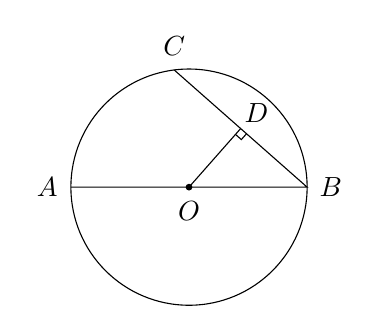
\begin{tikzpicture}
      \filldraw (0,0) circle (1pt);
      \draw (0,0) circle (1.5cm);
      \draw (-.188,1.488) -- (1.5,0) -- (-1.5,0);
      \draw (.656,.744) -- (0,0);
      \draw (.59,.67) -- (.665,.604) -- (.730,.678);
      \node at (0,-.3) {$O$};
      \node at (-1.8,0) {$A$};
      \node at (1.8,0) {$B$};
      \node at (-.188,1.788) {$C$};
      \node at (.856,.944) {$D$};
    \end{tikzpicture}
    \vspace*{-1ex}
    \caption*{圖(九)}
    \vspace*{-2ex}
  \end{figure}
  \begin{choices}
    \item $6\sqrt{7}$
    \item $12\sqrt{7}$
    \item $15$
    \item $30$
  \end{choices}
\end{problem}
\end{document}
